\documentclass[11pt]{article}

\usepackage[margin=2.5cm]{geometry}
\usepackage{graphicx}
\usepackage{booktabs}
\usepackage{hyperref}
\usepackage[numbers,square,sort&compress]{natbib}
\usepackage{lineno}
\usepackage{setspace}
\usepackage{authblk}
\usepackage{amsmath}
\usepackage{xcolor}
\usepackage{caption}
\emergencystretch=3em

\linenumbers
\doublespacing
% Auto-generated by scripts/summarize_results.py; do not edit manually.
\newcommand{\AllSixPatternN}{19}
\newcommand{\CanonicalApprisDifferentN}{2631}
\newcommand{\CanonicalLegacyDifferentN}{4596}
\newcommand{\CjGenomePamN}{21590}
\newcommand{\CjGenomePamPct}{100.0}
\newcommand{\CjHomeostaticTargetN}{30}
\newcommand{\CjHomeostaticTargetPct}{54.5}
\newcommand{\CjLLTolerizedTargetN}{37}
\newcommand{\CjLLTolerizedTargetPct}{67.3}
\newcommand{\CjPLAcuteLPSTargetN}{39}
\newcommand{\CjPLAcuteLPSTargetPct}{70.9}
\newcommand{\CjPPControlTargetN}{35}
\newcommand{\CjPPControlTargetPct}{63.6}
\newcommand{\CjPanelPamN}{55}
\newcommand{\CjPanelPamPct}{100.0}
\newcommand{\CjShamTargetN}{37}
\newcommand{\CjShamTargetPct}{67.3}
\newcommand{\CjStrokeTargetN}{42}
\newcommand{\CjStrokeTargetPct}{76.4}
\newcommand{\FripMax}{0.61}
\newcommand{\FripMin}{0.25}
\newcommand{\MultiStudyPatternN}{15}
\newcommand{\NGene}{21599}
\newcommand{\NPanel}{55}
\newcommand{\NRun}{13}
\newcommand{\NmeGenomePamN}{21568}
\newcommand{\NmeGenomePamPct}{99.9}
\newcommand{\NmeHomeostaticTargetN}{30}
\newcommand{\NmeHomeostaticTargetPct}{54.5}
\newcommand{\NmeLLTolerizedTargetN}{37}
\newcommand{\NmeLLTolerizedTargetPct}{67.3}
\newcommand{\NmePLAcuteLPSTargetN}{39}
\newcommand{\NmePLAcuteLPSTargetPct}{70.9}
\newcommand{\NmePPControlTargetN}{35}
\newcommand{\NmePPControlTargetPct}{63.6}
\newcommand{\NmePanelPamN}{55}
\newcommand{\NmePanelPamPct}{100.0}
\newcommand{\NmeShamTargetN}{37}
\newcommand{\NmeShamTargetPct}{67.3}
\newcommand{\NmeStrokeTargetN}{42}
\newcommand{\NmeStrokeTargetPct}{76.4}
\newcommand{\NoContextPatternN}{16}
\newcommand{\PanelClassSpreadMaxPP}{14.5}
\newcommand{\PanelClassSpreadMinPP}{10.9}
\newcommand{\SaGenomePamN}{21211}
\newcommand{\SaGenomePamPct}{98.2}
\newcommand{\SaHomeostaticTargetN}{25}
\newcommand{\SaHomeostaticTargetPct}{45.5}
\newcommand{\SaLLTolerizedTargetN}{35}
\newcommand{\SaLLTolerizedTargetPct}{63.6}
\newcommand{\SaPLAcuteLPSTargetN}{37}
\newcommand{\SaPLAcuteLPSTargetPct}{67.3}
\newcommand{\SaPPControlTargetN}{32}
\newcommand{\SaPPControlTargetPct}{58.2}
\newcommand{\SaPanelPamN}{53}
\newcommand{\SaPanelPamPct}{96.4}
\newcommand{\SaShamTargetN}{36}
\newcommand{\SaShamTargetPct}{65.5}
\newcommand{\SaStrokeTargetN}{39}
\newcommand{\SaStrokeTargetPct}{70.9}
\newcommand{\SensitivityMaxChanged}{16}
\newcommand{\SensitivityMaxDeltaPP}{29.1}
\newcommand{\SingleStudyPatternN}{5}
\newcommand{\SpGenomePamN}{21593}
\newcommand{\SpGenomePamPct}{100.0}
\newcommand{\SpHomeostaticTargetN}{31}
\newcommand{\SpHomeostaticTargetPct}{56.4}
\newcommand{\SpLLTolerizedTargetN}{37}
\newcommand{\SpLLTolerizedTargetPct}{67.3}
\newcommand{\SpPLAcuteLPSTargetN}{39}
\newcommand{\SpPLAcuteLPSTargetPct}{70.9}
\newcommand{\SpPPControlTargetN}{35}
\newcommand{\SpPPControlTargetPct}{63.6}
\newcommand{\SpPanelPamN}{55}
\newcommand{\SpPanelPamPct}{100.0}
\newcommand{\SpShamTargetN}{37}
\newcommand{\SpShamTargetPct}{67.3}
\newcommand{\SpStrokeTargetN}{42}
\newcommand{\SpStrokeTargetPct}{76.4}
\newcommand{\TSSEnrichMax}{31.4}
\newcommand{\TSSEnrichMin}{20.3}
\newcommand{\TfeThreeCanonicalTSS}{7628896}
\newcommand{\TfeThreeLegacyOffset}{0}
\newcommand{\TfeThreeLegacyTSS}{7628896}
\newcommand{\TfeThreeUnContextsN}{6}
\newcommand{\TfeThreeUnPamN}{3}
\newcommand{\TfebCanonicalTSS}{48096644}
\newcommand{\TfebLegacyOffset}{48690}
\newcommand{\TfebLegacyTSS}{48047954}
\newcommand{\TfebUnContextsN}{0}
\newcommand{\TfebUnPamN}{5}
\newcommand{\UnGenomePamN}{20022}
\newcommand{\UnGenomePamPct}{92.7}
\newcommand{\UnGenomeTargetMaxPct}{43.3}
\newcommand{\UnGenomeTargetMinPct}{29.0}
\newcommand{\UnHomeostaticTargetN}{23}
\newcommand{\UnHomeostaticTargetPct}{41.8}
\newcommand{\UnLLTolerizedTargetN}{31}
\newcommand{\UnLLTolerizedTargetPct}{56.4}
\newcommand{\UnPLAcuteLPSTargetN}{33}
\newcommand{\UnPLAcuteLPSTargetPct}{60.0}
\newcommand{\UnPPControlTargetN}{28}
\newcommand{\UnPPControlTargetPct}{50.9}
\newcommand{\UnPanelAcrossContextRangePP}{23.6}
\newcommand{\UnPanelPamN}{50}
\newcommand{\UnPanelPamPct}{90.9}
\newcommand{\UnPanelTargetMaxPct}{65.5}
\newcommand{\UnPanelTargetMinPct}{41.8}
\newcommand{\UnShamTargetN}{31}
\newcommand{\UnShamTargetPct}{56.4}
\newcommand{\UnStrokeTargetN}{36}
\newcommand{\UnStrokeTargetPct}{65.5}


\begin{document}

\title{A genome-wide, guide-site-aware CRISPRa targetability dataset and prioritization framework for murine microglial ATAC-seq contexts}
\author[1,2,*]{Ernest Darell Zerme\~no}
\affil[1]{Universidad Panamericana, Guadalajara, Mexico}
\affil[2]{Centro Universitario de Ciencias Biol\'ogicas y Agropecuarias, Universidad de Guadalajara, Zapopan, Mexico}
\affil[*]{Correspondence: 0244552@up.edu.mx; ORCID: 0009-0002-1721-4526}
\date{}
\maketitle

\begin{abstract}
\textbf{Background:} Compact CRISPR-mediated transcriptional activation (CRISPRa) systems can ease adeno-associated virus packaging constraints, but their restricted protospacer-adjacent motifs (PAMs) and the chromatin environment of the actual guide site both affect candidate selection. Existing design tools are general purpose; to our knowledge, a reproducible resource focused on microglial regulatory contexts has been lacking.

\textbf{Results:} We uniformly reprocessed \NRun{} public murine microglial ATAC-seq runs from three studies and scanned the transcription-oriented $-400$ to $-50$ bp promoter window of 21,599 GENCODE vM33 protein-coding genes. The resource represents five distinct nuclease/PAM classes across six modelled CRISPRa configurations; HEAL and SminiCRa share the Un1Cas12f1 TTTR targeting class, and the dNme2Cas9 activator is a sequence-level proposed configuration. Unlike a promoter-midpoint proxy, the primary definition requires the complete protospacer plus PAM interval to be contained in a primary ATAC peak. In a frozen 55-gene therapeutic panel, \UnPanelPamN/55 genes (\UnPanelPamPct\%) contained a sequence-filtered TTTR candidate, whereas \UnPanelTargetMinPct--\UnPanelTargetMaxPct\% had a complete Un1Cas12f1 guide site supported across individual dataset contexts. The corresponding genome-wide range was \UnGenomeTargetMinPct--\UnGenomeTargetMaxPct\%. \textit{Tfeb} and \textit{Tfe3} had TTTR candidates but primary peak support in \TfebUnContextsN/6 and \TfeThreeUnContextsN/6 contexts, respectively. Canonical-TSS, APPRIS, legacy-TSS, matched-depth, and Genrich/MACS3 analyses showed explicitly which calls were definition-sensitive. Across-study differences remained descriptive because study, isolation, sequencing, depth, and biology were confounded. An exploratory 53-gene human ortholog-panel check across two independent iPSC-/hPSC-derived microglia ATAC-seq datasets reproduced the selected-promoter \textit{TFE3}/\textit{TFEB} qualitative contrast, while also showing that \textit{TFEB} support is TSS-dependent.

\textbf{Conclusions:} PAM availability was broader than guide-site support in the promoter window studied. The resource provides auditable candidate protospacers and robustness annotations for experimental prioritization, not evidence of CRISPRa efficacy, non-activatability, safety, or therapeutic benefit.
\end{abstract}

\noindent\textbf{Keywords:} CRISPRa; microglia; ATAC-seq; chromatin accessibility; guide design; Cas12f; PAM; targetability dataset

\section{Background}

CRISPR-mediated transcriptional activation (CRISPRa) increases endogenous gene expression without introducing a targeted double-strand break. Its use in vivo is constrained by delivery: the coding sequence of SpCas9 alone occupies much of the approximately 4.7-kb adeno-associated virus payload, motivating smaller effectors and activation architectures \citep{vora2018miniVPR,bohm2020crispra}. Compact systems based on Un1Cas12f1 and CjCas9 have demonstrated mammalian transcriptional activation, including HEAL, SminiCRa, and MiniCAFE \citep{wan2026heal,wang2024sminicra,zhang2021minicafe}. Compactness does not remove the need for an appropriately positioned PAM and protospacer.

Chromatin provides a second selection layer. CRISPRi/a activity depends strongly on guide position and local regulatory context, and established design frameworks already use chromatin data to prioritize guide RNAs \citep{horlbeck2016crispri,sanson2018crispra,crisprverse2022}. Accessibility is nevertheless probabilistic rather than a universal binary requirement: an ATAC-supported site is a more plausible candidate, while absence of an ATAC peak does not prove that a potent activator cannot engage the locus.

Microglia are especially relevant because their regulatory landscape responds to tissue environment and inflammatory history \citep{gosselin2017environment,wendeln2018innate,zhangx2022innate}. CRISPRi/a has also been implemented in human induced-pluripotent-stem-cell-derived microglia, establishing a practical route to functional follow-up \citep{drager2022crispri}. That platform is the closest functional microglia CRISPRi/a comparator; the present work instead provides a murine genome-wide promoter/PAM-by-ATAC prioritization matrix for compact CRISPRa design. Public murine ATAC-seq datasets span homeostatic, endotoxin-exposure, surgical-control, and stroke settings, but these datasets were generated by different laboratories with different isolation and sequencing strategies. They can support a multi-context resource, not a balanced causal comparison of ``microglial states.''

Here we rebuild a genome-wide murine microglial targetability dataset around the coordinate that matters experimentally: the complete protospacer--PAM interval. We distinguish five targeting classes across six modelled CRISPRa configurations, define TSS and peak-set provenance, use independent biological replicates where available, label technical-only contexts, and quantify sensitivity to depth, peak caller, TSS choice, and operational definition. The contribution is a transparent resource for prioritizing experiments rather than a new guide-scoring algorithm or a claim of functional activation.

\section{Results}

\subsection{The revised resource makes guide position, TSS choice, and replication explicit}

The workflow starts from checksum-verified FASTQs and GENCODE vM33 rather than inherited peak files (Figure~1). It includes 21,599 nuclear protein-coding genes, \NRun{} sequencing runs, six dataset contexts, and a frozen 55-gene panel. Ensembl-canonical transcripts define the primary TSS. APPRIS selected a different TSS for \CanonicalApprisDifferentN{} genes and the previous most-5-prime GENCODE-basic rule differed for \CanonicalLegacyDifferentN{} genes, demonstrating that TSS selection is not a bookkeeping detail.

Five nuclease/PAM classes are evaluated (Table~1). HEAL and SminiCRa both use Un1Cas12f1 with a TTTR PAM, so their sequence and ATAC-based targeting matrices are identical even though their scaffolds and activation architectures differ. They are consequently represented as two configurations but one targeting class. Nme2Cas9 contributes a compact, experimentally established N$_4$CC DNA-targeting rule, but the dNme2Cas9 activator entry is a proposed configuration rather than a validated CRISPRa platform \citep{edraki2019nme2}.

For biologically replicated inputs, the primary peak set retains sequence supported by a qualifying pair of independent replicate peaks at 50\% reciprocal overlap. The intersection of each qualifying pair makes complete guide containment conservative. The PBS/PBS, PBS/LPS, and LPS/LPS inputs consist of paired technical runs from a single biological preparation per condition; they are pooled and explicitly carry no biological-reproducibility claim.

\subsection{Sequence-level PAM coverage is broad in the surveyed promoter window}

Both strands of the $-400$ to $-50$ bp window were scanned with IUPAC-aware PAM matching and class-specific spacer lengths. Candidates passed prespecified GC, homopolymer, and cloning-site filters. Across the genome, \UnGenomePamN{} of 21,599 promoters (\UnGenomePamPct\%) contained at least one passing Un1Cas12f1 TTTR candidate (Figure~2A). Coverage of the frozen panel was \UnPanelPamN/55 (\UnPanelPamPct\%; Figure~2B); the corresponding values were \SaPanelPamPct\%, \SpPanelPamPct\%, \CjPanelPamPct\%, and \NmePanelPamPct\% for SaCas9, SpCas9, CjCas9, and Nme2Cas9. These values quantify sequence availability within the chosen window; they do not predict expression gain.

Candidate abundance varied substantially among PAM classes (Figure~2D). This was expected from motif degeneracy and spacer filtering, and it is why the main comparison is not simply whether a promoter contains a motif. To report multi-class coverage explicitly, we added a class-multiplicity summary. At the sequence layer, \MultiGenomeSeqAllFiveN/21,599 genome-wide genes and \MultiPanelSeqAllFiveN/55 panel genes contained passing candidates for all five targeting classes; only \MultiGenomeSeqOneN{} genome-wide genes had candidates for exactly one class and \MultiGenomeSeqNoneN{} had none. The relevant prioritization question is whether a specific complete candidate interval has reproducible ATAC support.

\subsection{Complete guide-site support narrows broad PAM availability into context-specific candidate sets}

The primary call requires at least one complete protospacer plus PAM interval to be fully contained in the applicable primary peak. For Un1Cas12f1, \UnPanelTargetMinPct--\UnPanelTargetMaxPct\% of the frozen panel met this rule across the six individual contexts, compared with \UnPanelPamPct\% at the sequence-only layer (Figure~3A). Genome-wide Un1Cas12f1 guide-site support ranged from \UnGenomeTargetMinPct\% to \UnGenomeTargetMaxPct\% (Figure~2C).

Within a context, the range among the five nuclease/PAM classes was \PanelClassSpreadMinPP--\PanelClassSpreadMaxPP{} percentage points in the panel. Across contexts, the Un1Cas12f1 range was \UnPanelAcrossContextRangePP{} percentage points. This does \emph{not} establish that biological state has a larger effect than nuclease choice: the cross-context range also contains laboratory, sorting, sequencing-layout, depth, and population-composition differences. Accordingly, Figures~2 and 3 label the six columns by study and treatment rather than presenting them as exchangeable states.

The guide-by-context heatmap gives the intended use of the resource (Figure~3C): it separates genes with sequence-only candidates from genes with complete, context-supported guide intervals that can be carried forward to experimental testing. A positive cell means that at least one candidate interval satisfies the primary rule in that context. A negative cell means only that no candidate passed this particular sequence, window, TSS, peak, and containment definition.

The multiplicity pattern changed after adding the primary ATAC criterion. Considering support in any surveyed context, \MultiGenomeAnyAllFiveN/21,599 genome-wide genes and \MultiPanelAnyAllFiveN/55 panel genes had primary guide-site support for all five targeting classes, whereas \MultiGenomeAnyNoneN{} genome-wide genes and \MultiPanelAnyNoneN{} panel genes had no primary support for any class. Per-context multiplicity distributions are reported in Table~S7.

\subsection{TSS, containment, depth, and peak caller expose definition-sensitive loci}

Four operational quantities were kept separate: complete guide containment, any guide/peak overlap, promoter-midpoint coverage, and any promoter/peak overlap (Supplementary Figure~S3). They answer different questions and produced different estimates; promoter overlap was not relabelled as guide targetability.

TSS choice had a locus-specific impact. The Ensembl-canonical and legacy TSSs for \textit{Tfeb} differed by \TfebLegacyOffset{} bp, whereas the corresponding \textit{Tfe3} definitions differed by \TfeThreeLegacyOffset{} bp (Figure~4C). Under the canonical primary analysis, \textit{Tfeb} contained \TfebUnPamN{} passing TTTR candidates and had guide-site support in \TfebUnContextsN/6 contexts; \textit{Tfe3} contained \TfeThreeUnPamN{} and had support in \TfeThreeUnContextsN/6. These are target-selection hypotheses, not evidence that either paralog is functionally superior. The distinction matters because TFEB and related MiT/TFE factors regulate lysosomal programs, but abundance, localization, occupancy, and downstream function cannot be inferred from promoter ATAC alone \citep{sardiello2009gene,settembre2011tfeb,iyer2022lysosomal}.

To evaluate sequencing depth and caller dependence without discarding replication structure, biological inputs were downsampled at replicate level to an equal condition-total target, called per replicate, and reconstructed with the same replicate-consensus rule. Technical-only contexts were downsampled after cross-lane pooling and duplicate removal. Genrich and MACS3 were then evaluated in parallel. Across the TSS, depth, and caller variants, the largest change relative to a primary panel call affected \SensitivityMaxChanged{} genes in a class--context cell, corresponding to \SensitivityMaxDeltaPP{} percentage points (Supplementary Figure~S4). The Jaccard index of promoters overlapped by each caller and binary promoter-call concordance are reported separately (Supplementary Figure~S6), rather than justifying Genrich from a local software failure.

\subsection{Evidence provenance enables candidate prioritization without causal state labels}

For Un1Cas12f1, \AllSixPatternN{} panel genes had guide-site support in all six contexts, \MultiStudyPatternN{} had support in at least two studies without being positive in every context, \SingleStudyPatternN{} were supported within one study, and \NoContextPatternN{} had no support under the surveyed primary definitions (Figure~4A). These labels replace causal categories such as ``inflammation-gained'' or ``injury-open.'' A within-panel Fisher analysis evaluated whether these support patterns were associated with the functional labels used to curate the panel, with Benjamini--Hochberg adjustment across the full test family (Supplementary Figure~S5). It was treated as descriptive because the panel and its categories were selected a priori.

Candidate Table~S3 reports the selected transcript, TSS, spacer and PAM coordinates, strand, distance to TSS, supporting peak identifier and signal in each context, distance to the peak summit, and the number of positive contexts. A normalized candidate-by-run companion table reports complete and partial support, run-level peak identifier, signal, and summit distance, preserving the distinction between biological replicates and technical lanes. The first five candidates per gene and targeting class are presented as candidate protospacers rather than recommendations. This format converts the matrix into a triage list: a user can select candidates with explicit TSS, peak, replicate, signal, and off-target provenance before functional CRISPRa testing. The Un1Cas12f1 subset additionally received exhaustive Bowtie alignment through three mismatches followed by an orientation-aware TTTR check and exon/canonical-promoter annotation (Figure~5). That screen does not model bulges, cleavage, nuclease-specific mismatch energetics, chromatin at off-targets, or experimental genotoxicity.

\subsection{Matched-promoter analysis separates panel composition from random genomic placement}

The previous comparison with peaks shuffled uniformly across the genome was replaced because open-chromatin peaks are naturally promoter enriched. For each frozen-panel promoter, non-panel promoters were matched using promoter GC decile, annotated transcript-count bin, and number of passing Un1Cas12f1 candidates. Ten thousand matched panels were sampled with seed 1729 (Supplementary Figure~S7). The analysis compares this curated panel with sequence- and annotation-matched promoters; it is not functional validation and could not additionally match expression or mappability across every context.

\subsection{Human ortholog-panel checks test whether selected prioritization patterns persist in independent microglia-like datasets}

To address whether selected prioritization patterns were specific to the murine datasets, we performed an exploratory human ortholog-panel check using processed ATAC-seq peaks from two independent human iPSC-/hPSC-derived microglia resources \citep{yang2023advariants,booms2024pdrisk}. The locked 55-gene mouse panel mapped to 53 human symbols for this check; \textit{Siglech} and \textit{Chil3} were excluded because a direct one-to-one human ortholog was not used. GENCODE v19/hg19 promoters were selected with the same deterministic APPRIS/CCDS/basic/TSL/length rule used for the check, and the same PAM classes, sequence filters, promoter window, and complete-site-in-peak primary rule were applied.

In GSE206479, any-context strict targetability across the 53 mapped genes was 32/53 for Un1Cas12f1, 38/53 for SaCas9, and 42/53 for SpCas9, CjCas9, and Nme2Cas9. In the independent GSE245522 peak sets, any-replicate support was lower (20/53, 29/53, 36/53, 35/53, and 36/53, respectively), and requiring a guide site to be supported in at least three of four peak files gave 15/53, 21/53, 29/53, 26/53, and 26/53. Thus the exact targetability fraction was dataset-dependent, but the qualitative pattern that ATAC support narrows sequence-level PAM availability was retained.

As a worked example of hypothesis generation, the selected human \textit{TFE3} promoter was supported in every GSE206479 context and every GSE245522 replicate for all five PAM classes. The selected human \textit{TFEB} promoter lacked support in both datasets for all five PAM classes despite containing sequence-filtered candidates. However, a transcript-level sensitivity analysis showed that alternative GENCODE v19 \textit{TFEB} TSS choices can be accessible. This human check therefore supports a concrete cross-dataset hypothesis for follow-up, but it is not CRISPRa validation and should not be read as a gene-wide claim that human \textit{TFEB} cannot be targeted.

Together, these analyses show that the revised resource is most useful as an evidence-preserving prioritization framework: broad promoter PAM availability is filtered by exact guide-site accessibility, TSS choice, replicate support, peak-calling choices, and dataset provenance before any functional claim is made.

\section{Discussion}

This revision changes the scientific object from a promoter-level proxy to a guide-site resource. The old midpoint rule could reject a fully accessible candidate because a peak failed to cover $-225$ bp, or accept promoter accessibility without proving that any complete candidate was supported. Requiring the complete spacer--PAM interval removes that mismatch while preserving midpoint and overlap quantities as transparent sensitivities.

The broad sequence coverage of compact PAM classes is useful but unsurprising in a 350-bp, two-strand search. The more informative output is the identity and robustness of individual sites after integrating public microglial ATAC-seq. ATAC support is not a universal binary determinant. Nucleosome breathing, activator potency, chromatin remodelers, and experimental context can permit activity where a peak caller reports no peak. Conversely, an accessible site can fail because of guide folding, effector geometry, delivery, expression, or biological feedback. ``Targetable'' is therefore an operational resource label, and candidate-site plausibility is the more general interpretation.

The multi-context design has a deliberate limit. The three studies were not a joint experiment. Gosselin used ex vivo homeostatic microglia and single-end sequencing; Zhang X/Kracht assessed endotoxin exposure with technical sequencing runs; Zhang and colleagues profiled separate sham and stroke animals using a different isolation strategy. Downsampling, a shared peak universe, and a second caller diagnose some technical sensitivity but cannot remove study confounding. The strongest comparisons are those internal to the Zhang X/Kracht and sham--stroke series, while consistency across laboratories is useful as robustness evidence rather than a causal state effect.

The revised \textit{Tfeb}/\textit{Tfe3} example illustrates why the additional safeguards matter. A large alternative-TSS displacement can move the entire 350-bp search window to another locus segment. Primary support for one paralog across more contexts would still not demonstrate greater activation, lysosomal flux, or therapeutic benefit. The human ortholog-panel check sharpened this point rather than eliminating it: the selected \textit{TFE3} promoter was consistently supported across two human iPSC-/hPSC-derived microglia datasets, but the selected \textit{TFEB} result was TSS-dependent when alternative GENCODE v19 transcripts were examined. The resource therefore defines a direct experiment: select candidates with explicit TSS and peak support, activate endogenous \textit{Tfeb}/\textit{TFEB} and \textit{Tfe3}/\textit{TFE3} side by side in an appropriate microglial system, and measure transcriptional engagement and function.

Several limitations remain. The promoter window is standardized rather than transcript- and cell-state-optimized. Canonical/APPRIS annotations are proxies for the expressed TSS, because matched microglial CAGE data were unavailable across all contexts. Replicate-consensus peaks increase specificity at the cost of sensitivity. Three contexts lack biological replicates. ATAC signal is relative and peak-caller dependent. The 55-gene panel is curated rather than randomly sampled, so its resampling intervals measure stability of that fixed panel rather than population inference. The promoter-matched null lacks expression and mappability matching. Candidate scores are heuristic for Un1Cas12f1, and off-target analysis remains preliminary. The human ortholog check is limited to iPSC-/hPSC-derived microglia datasets, does not compare equivalent mouse and human biological states, and does not replace genome-wide human reconstruction or CRISPRa validation. Finally, all primary resource results are murine and computational; direct CRISPRa and functional validation are required.

\section{Conclusions}

Within a standardized murine promoter window, PAM-bearing candidates were common, whereas complete guide sites supported by primary microglial ATAC peaks were less frequent and definition dependent. The revised resource makes those dependencies visible at guide resolution and provides exact candidates, peak provenance, TSS alternatives, quality controls, and caller/depth sensitivities. It should be used to prioritize experiments, not to infer efficacy or rule out loci.

\section{Methods}

\subsection{Study design and frozen panel}

The analysis was designed as a predictive genomics resource. A pre-existing 55-gene panel covering autophagy/lysosome, inflammation, phagocytosis, lipid metabolism, neuroprotection, microglial identity, and epigenetic regulation was frozen in \texttt{config/therapeutic\_genes\_locked.csv} before the present reanalysis. Genes were included because they represented recurring microglial programs with experimental or therapeutic relevance, including MiT/TFE and lysosomal biology \citep{sardiello2009gene,settembre2011tfeb,iyer2022lysosomal}, innate immune memory and inflammatory regulation \citep{wendeln2018innate,zhangx2022innate}, and microglial identity or functional screening contexts \citep{gosselin2017environment,drager2022crispri}. Row-level categories, priorities, and literature-linked justifications are recorded in Table~S1. No gene was added or removed based on the revised targetability results. The panel is a complete curated set of interest, not a random sample of therapeutic genes. Genome-wide results are therefore reported alongside panel summaries.

\subsection{Reference genome, transcript selection, and promoter windows}

The workflow downloads GRCm39/mm39 from UCSC and GENCODE mouse vM33 annotations \citep{frankish2021gencode}. Nuclear protein-coding transcripts were grouped by gene symbol. The primary transcript was tagged \texttt{Ensembl\_canonical}; genes without that tag used APPRIS principal, then a GENCODE-basic fallback with transcript-support level and length as deterministic tie breakers. Sensitivities independently selected APPRIS principal and the most 5-prime GENCODE-basic transcript. Every selection, fallback, transcript identifier, strand, TSS, tag set, and transcript count is recorded in \texttt{reference/tss\_selection.tsv}.

TSSs use zero-based genomic coordinates. The promoter search interval was $-400$ to $-50$ bp in transcriptional orientation: \texttt{[TSS-400,TSS-50)} on the positive strand and the corresponding downstream genomic coordinates on the negative strand.

\subsection{Nuclease/PAM classes and candidate scanning}

Five distinct targeting classes were scanned (Table~1). PAM and spacer rules followed the corresponding experimental literature \citep{friedland2015sa,zhang2021minicafe,edraki2019nme2,wang2024sminicra}. Overlapping PAM matches were detected on both strands using full IUPAC reverse complements. Class-specific spacers were extracted only when the full spacer and PAM fell within the promoter window. Protospacers were retained at 30--70\% GC, with no homopolymer longer than four nucleotides and no BsmBI or BsaI recognition site in either orientation. Candidate counts therefore refer to sequence-filtered protospacers, not raw PAM occurrences. Only Un1Cas12f1 candidates received a simple heuristic score based on GC balance, homopolymer length, and poly-T avoidance; no validated efficacy model was claimed.

\subsection{Public ATAC-seq inputs}

Thirteen runs were obtained from ENA using URLs and MD5 checksums frozen in \path{config/samples.tsv} (Table~2). The Gosselin dataset comprised two independent single-end homeostatic microglial runs (GSE89960) \citep{gosselin2017environment}. The Zhang X/Kracht dataset comprised paired technical runs for PBS/PBS, PBS/LPS, and LPS/LPS preparations (GSE175578) \citep{zhangx2022innate}. The Zhang dataset comprised two sham and three stroke biological replicates (GSE220041) \citep{zhang2024hdac3stroke}.

\subsection{ATAC-seq processing and quality control}

ATAC-seq processing followed established principles \citep{buenrostro2013atacseq,corces2017omni}. Adapters were removed with Trim Galore 0.6.10 \citep{krueger2015trimgalore}. Reads were aligned with Bowtie2 2.5.4 in \texttt{--very-sensitive} mode; paired-end data additionally used \texttt{--maxins 1000 --no-mixed --no-discordant} \citep{langmead2012bowtie2}. BAMs were sorted with SAMtools 1.21, duplicate fragments removed with Picard 3.3, and alignments filtered to MAPQ $\geq30$, proper pairs for paired-end data, primary/non-supplementary alignments, and non-mitochondrial sequence \citep{li2009samtools,quinlan2010bedtools}. Optical-duplicate inference was disabled because ENA/SRA read identifiers do not retain flowcell coordinates; coordinate-based duplicate removal was unchanged. Paired-end blacklist filtering removed the intact pair when either mate overlapped a blacklist interval. The official ENCODE mm10 v2 blacklist (ENCFF543DDX; SHA-256 \texttt{9638bbeb...bfac7}) was mapped with the UCSC mm10-to-mm39 chain: 3,360 of 3,435 intervals mapped and 75 did not; all source and mapped coordinates are recorded in \path{reference/blacklist_liftover_provenance.tsv} \citep{amemiya2019encode}. Genrich 0.6.1 was run in ATAC mode, which applies its ATAC cut-site adjustment internally; single-end data additionally used \texttt{-y} \citep{genrich2019}. Genrich was selected as the prespecified primary caller because it directly supports ATAC-seq, not because another caller failed locally.

Per-run QC comprised Bowtie2 overall alignment rate, usable fragment/read count, duplication metrics, replicate peak count, fraction of usable fragments or reads overlapping the run's peaks, fragment-length summaries for paired-end data, and maximum TSS enrichment from Tn5-adjusted insertion sites within $\pm2$ kb. FRiP reference lines are descriptive because library type and peak definition differ among datasets.

\subsection{Primary peaks and continuous shared-universe signal}

For Gosselin, sham, and stroke, peaks from distinct biological replicates were paired when reciprocal overlap was at least 0.50. Each qualifying pair contributed its intersected interval; overlapping intersections were merged without bridging unsupported gaps. Every retained base was therefore covered by at least one qualifying pair. For stroke, support in any two of three independent replicates was sufficient. For each technical-only Zhang X/Kracht preparation, filtered lanes were merged and deduplicated again at the pooled-library level so that a fragment duplicated across lanes was retained only once. Each technical pool was then called once, with an explicit absence of biological replication. This second deduplication was not applied across independent biological replicates.

Condition-level filtered BAMs were also merged to create CPM-normalized 10-bp bigWigs for visualization. A union of the six primary peak sets was merged into a shared peak universe, and read/fragment signal was quantified for every condition. This continuous layer supports inspection of peak-threshold effects but was not substituted for biological replication.

\subsection{Primary targetability and operational sensitivities}

For every gene, targeting class, and context, a candidate was primarily supported when its complete half-open genomic interval spanning the protospacer and PAM was contained within a primary peak. A gene-level primary call was positive when at least one candidate was supported. Separately stored sensitivities were: any partial candidate/peak overlap, promoter-midpoint coverage, and any promoter-window/peak overlap. The latter two are promoter-accessibility measures, not guide targetability.

Guide-level outputs include exact mm39 coordinates, strand, PAM, protospacer, TSS distance, transcript and TSS provenance, peak identifier, peak signal, overlap, and summit distance at both primary-context and individual-run levels. Up to five candidates per gene/class were ranked by the number of primary positive contexts, partial-overlap contexts, minimum available supporting signal, Un1Cas12f1 heuristic score where applicable, GC balance, preferred TSS distance, and coordinate. The ranking is predictive and does not constitute an experimental recommendation.

\subsection{Matched-depth and peak-caller sensitivities}

Filtered condition BAMs were counted as read units for single-end data and read-pair units for paired-end data. The minimum condition total was the common target. For biologically replicated contexts, this target was allocated as evenly as available depth permitted among the independent runs; each run was deterministically subsampled, called separately, and reduced to a two-replicate, 50\%-reciprocal-overlap consensus. Technical-only contexts were subsampled once after cross-lane pooling and duplicate removal. Requested and observed post-sampling totals and all deterministic seeds are reported. Peaks were called independently with Genrich and MACS3 3.0.2 \citep{zhang2008macs}. MACS3 used paired-end mode for paired libraries and a fixed shift/extension model for single-end libraries. The targetability matrix was rebuilt for both matched-depth peak sets. Caller concordance was summarized by the Jaccard index of promoter sets with any caller peak and by binary promoter-window concordance; no peak-interval Jaccard was claimed.

\subsection{Statistical summaries and robustness}

For each class--context cell, 10,000 percentile resamples of the 55-gene vector were generated with seed 1729. These are labelled fixed-panel resampling stability intervals and are not confidence intervals for a population of all therapeutic genes. PAM-bearing but unsupported counts were reported descriptively because primary guide support is nested within sequence availability.

For the matched-promoter null, promoter GC was calculated from mm39 and combined with the number of annotated transcripts and number of passing Un1Cas12f1 candidates. Non-panel genes were matched by GC decile, transcript-count bin, and protospacer-count bin, with nearest-neighbour fallback in standardized feature space when a stratum was sparse. Ten thousand non-replacement panels were drawn where possible. Empirical $p$ values used $(b+1)/(N+1)$. Expression and mappability were unavailable on a uniform gene-by-context basis and were not matching variables.

Functional-category associations used two-sided Fisher exact tests within the frozen 55-gene universe, with Benjamini--Hochberg correction across every pattern--category combination. TSS, matched-depth Genrich, and matched-depth MACS3 calls were compared directly with the canonical primary matrix to report changed genes and proportion differences.

\subsection{Exploratory human ortholog-panel ATAC check}

The human analysis was a post-review translational sanity check, not a second genome-wide resource. Mouse panel symbols were mapped to direct human symbols using the HGNC-conventional uppercase symbol where unambiguous, with recorded manual exceptions for \textit{Il4ra}/\textit{IL4R} and \textit{Map1lc3b}/\textit{MAP1LC3B}. \textit{Siglech} and \textit{Chil3} were excluded from this check because no direct one-to-one human ortholog was used. GENCODE v19/hg19 was used to select one promoter per mapped human gene by APPRIS principal, CCDS, GENCODE-basic, transcript-support level, and transcript length in deterministic order. Promoter sequences were fetched from UCSC, scanned with the same PAM classes, spacer lengths, GC, homopolymer, cloning-site, and $-400$ to $-50$ bp window rules, and intersected with processed hg19 narrowPeak files.

Two public human iPSC-/hPSC-derived microglia ATAC-seq resources were evaluated. GSE206479 contributed H1 and WTC11 resting and IFN-\(\beta\)-stimulated IDR peak files from Yang et al. \citep{yang2023advariants}. GSE245522 contributed four iPSC-derived microglia narrowPeak files from Booms et al. \citep{booms2024pdrisk}. A gene was counted as supported within a file or context when at least one complete protospacer--PAM interval was contained in the corresponding peak file. For GSE245522, both any-replicate and at-least-three-of-four replicate summaries were reported. Input URLs, row counts, byte counts, SHA-256 hashes, mapping exclusions, selected promoters, sequence checks, summary tables, candidate-site tables, and the \textit{TFEB} transcript-level TSS audit are stored under \path{analysis_stats/human_ortholog_atac/} and regenerated by \path{scripts/human_ortholog_atac_check.py}.

\subsection{Preliminary off-target screen}

Up to five reported Un1Cas12f1 candidates per panel gene were aligned exhaustively to mm39 with Bowtie 1.3.1 using up to three mismatches \citep{langmead2009bowtie}. Alignments were retained only when a correctly oriented TTTR PAM was present next to the aligned protospacer. The intended coordinate was removed, and remaining alignments were annotated for overlap with a GENCODE exon or a $\pm1$-kb canonical-TSS window. The screen does not evaluate bulges, chromatin, cleavage probability, or nuclease-specific safety and should be followed by purpose-built tools and experimental assays.

\subsection{Reproducibility and use of generative AI}

The full workflow is implemented in Snakemake 8.25 \citep{molder2021snakemake}. Software versions are pinned in \path{environment.yml}; accessions, MD5 checksums, random seeds, TSS choices, matched-depth realizations, caller concordance, shared-universe signal, source tables, and figure scripts are version controlled. Core regression tests cover promoter orientation, complete guide containment, IUPAC reverse complementation, and replicate-consensus behavior. The versioned code release and machine-readable output tables are identified in Data availability.

During revision, OpenAI ChatGPT and Codex were used for language editing, literature discovery, code drafting and refactoring, test design, and workflow documentation. The author inspected the primary sources, reviewed the code and outputs, corrected errors, and takes full responsibility for the manuscript and analysis. No generative-AI system is an author.

\section{Availability of data and materials}

Raw murine ATAC-seq data are publicly available under GSE89960, GSE175578, and GSE220041; exact ENA run URLs and MD5 checksums are in \path{config/samples.tsv}. The GRCm39 FASTA is downloaded from UCSC and GENCODE vM33 from GENCODE. The exploratory human ortholog-panel check used processed public peak files from GSE206479 and GSE245522; exact URLs, dimensions, and SHA-256 hashes are recorded in \path{analysis_stats/human_ortholog_atac/input_file_audit.tsv}. Source code, frozen configuration, source tables, figure code, the release manifest, selected derived peak and signal artifacts, and compressed public reference inputs are archived in GitHub release v2.1.1 (\url{https://github.com/Jefemaestro33/Paper0-CRISPRa-Targetability-Atlas/releases/tag/v2.1.1}) and Zenodo (\url{https://doi.org/10.5281/zenodo.21970941}). Raw FASTQs and derived murine BAMs/bigWigs are not stored in Git but are recreated by \path{workflow/Snakefile}.

\section*{Declarations}

\subsection*{Ethics approval and consent to participate}
No new animal or human participants, specimens, or interventions were used. This secondary computational analysis used public, de-identified sequencing data generated under the approvals reported by the original studies.

\subsection*{Consent for publication}
Not applicable.

\subsection*{Competing interests}
The author declares no competing interests.

\subsection*{Funding}
This research received no external funding.

\subsection*{Authors' contributions}
E.D.Z. conceived the study, curated the target panel, designed and implemented the workflow, performed the analysis, interpreted the results, and wrote and revised the manuscript.

\subsection*{Acknowledgements}
The author thanks the investigators who generated and publicly released the ATAC-seq datasets used here.

\section*{Abbreviations}
ATAC-seq, assay for transposase-accessible chromatin using sequencing; CRISPRa, CRISPR-mediated transcriptional activation; FRiP, fraction of reads in peaks; PAM, protospacer-adjacent motif; TSS, transcription start site.

\section*{Additional files}

\begin{description}
\item[Table S1.] Frozen 55-gene panel, functional metadata, and descriptive guide-site support pattern.
\item[Table S2.] Complete genome-wide gene $\times$ targeting-class $\times$ context targetability matrix, including sequence counts and every operational accessibility definition.
\item[Table S3.] Candidate protospacers with exact TSS, interval, peak, context, and preliminary off-target annotations; accompanying run-level peak-evidence and full PAM-valid alignment tables.
\item[Table S4.] Per-run ATAC-seq quality control and primary-peak provenance.
\item[Table S5.] Descriptive cross-context Un1Cas12f1 support patterns for the frozen panel.
\item[Table S6.] Original mm10 and lifted mm39 ENCODE blacklist intervals.
\item[Table S7.] Fixed-panel stability, PAM-to-guide-site attrition, Cas-class multiplicity, matched-promoter null, and sensitivity records.
\end{description}

\bibliographystyle{unsrtnat}
\bibliography{references}

\clearpage
\begin{table}[p]
\centering
\caption{Targeting classes and represented modelled CRISPRa configurations. HEAL and SminiCRa share one targeting class; the dNme2Cas9 activator is proposed rather than experimentally validated.}
\label{tab:classes}
\small
\begin{tabular}{llll}
\toprule
Targeting class & PAM & Spacer & Represented configuration(s) \\
\midrule
Un1Cas12f1 & TTTR, 5-prime & 20 nt & HEAL; SminiCRa \\
SaCas9 & NNGRRT, 3-prime & 21 nt & SaCas9 CRISPRa \\
SpCas9 & NGG, 3-prime & 20 nt & SpCas9 CRISPRa \\
CjCas9 & NNNVRYM, 3-prime & 22 nt & MiniCAFE \\
Nme2Cas9 & NNNNCC, 3-prime & 24 nt & proposed dNme2Cas9 activator \\
\bottomrule
\end{tabular}
\end{table}

\begin{table}[p]
\centering
\caption{Public ATAC-seq inputs. ``Context'' is descriptive and does not imply a balanced cross-study state comparison.}
\label{tab:inputs}
\small
\begin{tabular}{lllll}
\toprule
Study & Context & Runs & Layout & Replication used \\
\midrule
Gosselin 2017 & ex vivo homeostatic & 2 & single-end & biological \\
Zhang X/Kracht 2022 & PBS/PBS & 2 & paired-end & technical \\
Zhang X/Kracht 2022 & PBS/LPS & 2 & paired-end & technical \\
Zhang X/Kracht 2022 & LPS/LPS & 2 & paired-end & technical \\
Zhang 2024 & sham & 2 & paired-end & biological \\
Zhang 2024 & stroke & 3 & paired-end & biological \\
\bottomrule
\end{tabular}
\end{table}

\section*{Figure legends}

\textbf{Figure 1. Corrected analysis architecture and scope.} Reference/TSS selection and five targeting classes are integrated with uniformly reprocessed public ATAC-seq. The primary call requires the complete protospacer plus PAM inside a primary peak.

\textbf{Figure 2. Sequence coverage and genome-wide guide-site support.} (A) Genome-wide and (B) frozen-panel promoters with at least one passing candidate. (C) Primary genome-wide calls by context and targeting class. (D) Candidate-count distributions.

\textbf{Figure 3. Sequence availability versus primary guide-site support.} (A) Un1Cas12f1 sequence coverage and complete-site support in the frozen panel. (B) Panel summaries for five targeting classes. (C) Gene-level Un1Cas12f1 matrix; this panel is intentionally restricted to Un1Cas12f1, while the other targeting classes are summarized in panel B and Table~S2. Teal cells indicate at least one fully contained candidate site and beige cells indicate no primary support. Red row labels mark the \textit{Tfeb}/\textit{Tfe3} examples. Between-context differences are descriptive.

\textbf{Figure 4. Descriptive panel patterns and TSS robustness.} (A) Cross-context support patterns. (B) \textit{Tfeb}/\textit{Tfe3} primary calls and promoter-overlap context; filled circles indicate complete guide-site support and red outlines indicate promoter-window overlap by a peak. (C) TSS offsets. (D) Call stability across TSS, depth, and caller variants.

\textbf{Figure 5. Evidence-aware candidate prioritization.} (A) Experimental-prioritization workflow. (B) Top Un1Cas12f1 \textit{Tfe3} candidates with supporting signal and preliminary PAM-aware off-target counts.

\textbf{Figure 6. Canonical-TSS-centered ATAC signal and guide evidence at \textit{Tfeb} and \textit{Tfe3}.} CPM-normalized signal within $\pm2.5$ kb, primary peak intervals, promoter windows, and supported candidate positions. All tracks use the corrected canonical TSS and primary peak rules. The six contexts share a y-axis scale within each gene column; the two gene columns are scaled independently.

\textbf{Supplementary Figure S1. Per-run ATAC-seq quality control.} Alignment, FRiP, TSS enrichment, and usable units; technical runs are visually distinguished from biological replicates.

\textbf{Supplementary Figure S2. Genome-wide candidate distributions and Un1Cas12f1 primary calls.}

\textbf{Supplementary Figure S3. Operational-definition sensitivity.} Complete containment, partial guide overlap, promoter-midpoint coverage, and any promoter overlap are shown separately.

\textbf{Supplementary Figure S4. TSS, depth, and peak-caller sensitivity of frozen-panel calls.}

\textbf{Supplementary Figure S5. Functional-category associations within the frozen 55-gene universe.}

\textbf{Supplementary Figure S6. Matched-depth Genrich/MACS3 concordance and deterministic sampling fractions.}

\textbf{Supplementary Figure S7. Promoter-matched null specification and results.}

\clearpage
\begin{figure}[p]\centering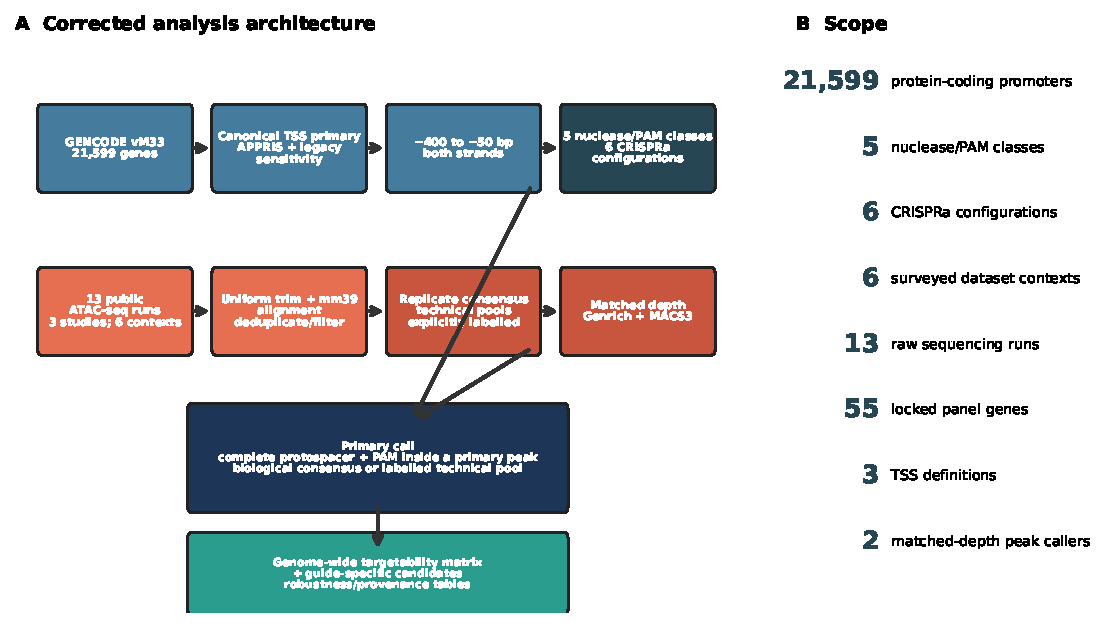
\includegraphics[width=\textwidth]{../figures/output/fig1.pdf}\caption*{Figure 1}\end{figure}
\clearpage
\begin{figure}[p]\centering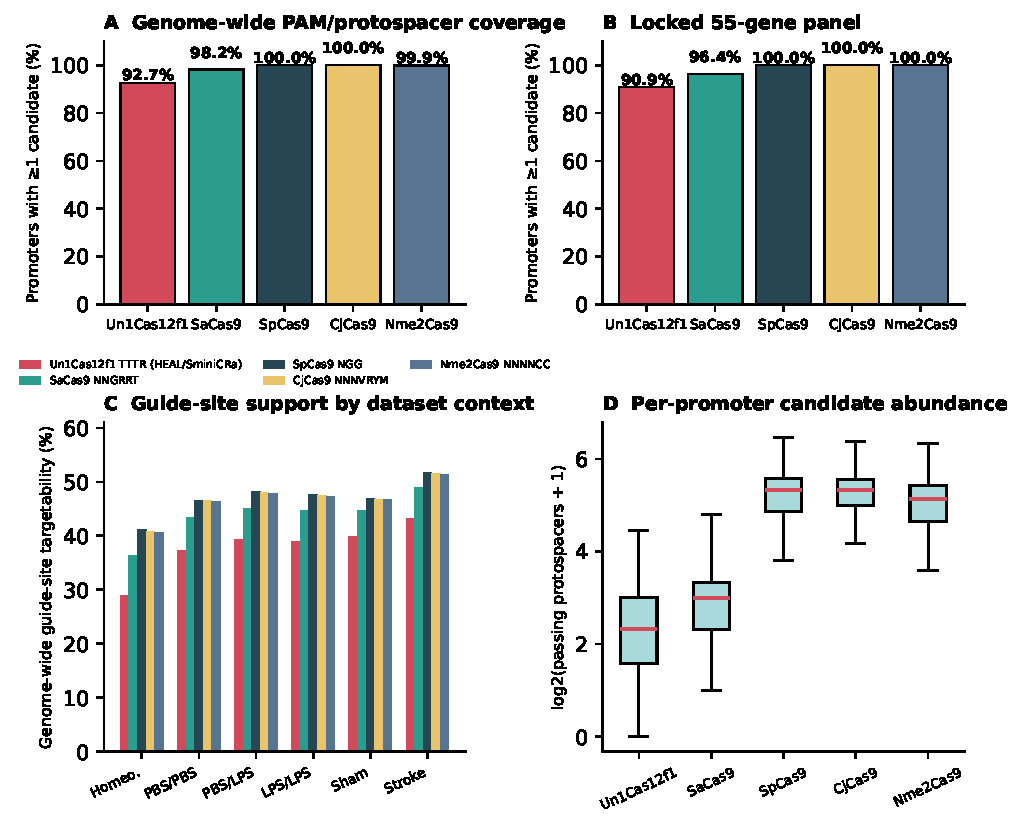
\includegraphics[width=\textwidth]{../figures/output/fig2.pdf}\caption*{Figure 2}\end{figure}
\clearpage
\begin{figure}[p]\centering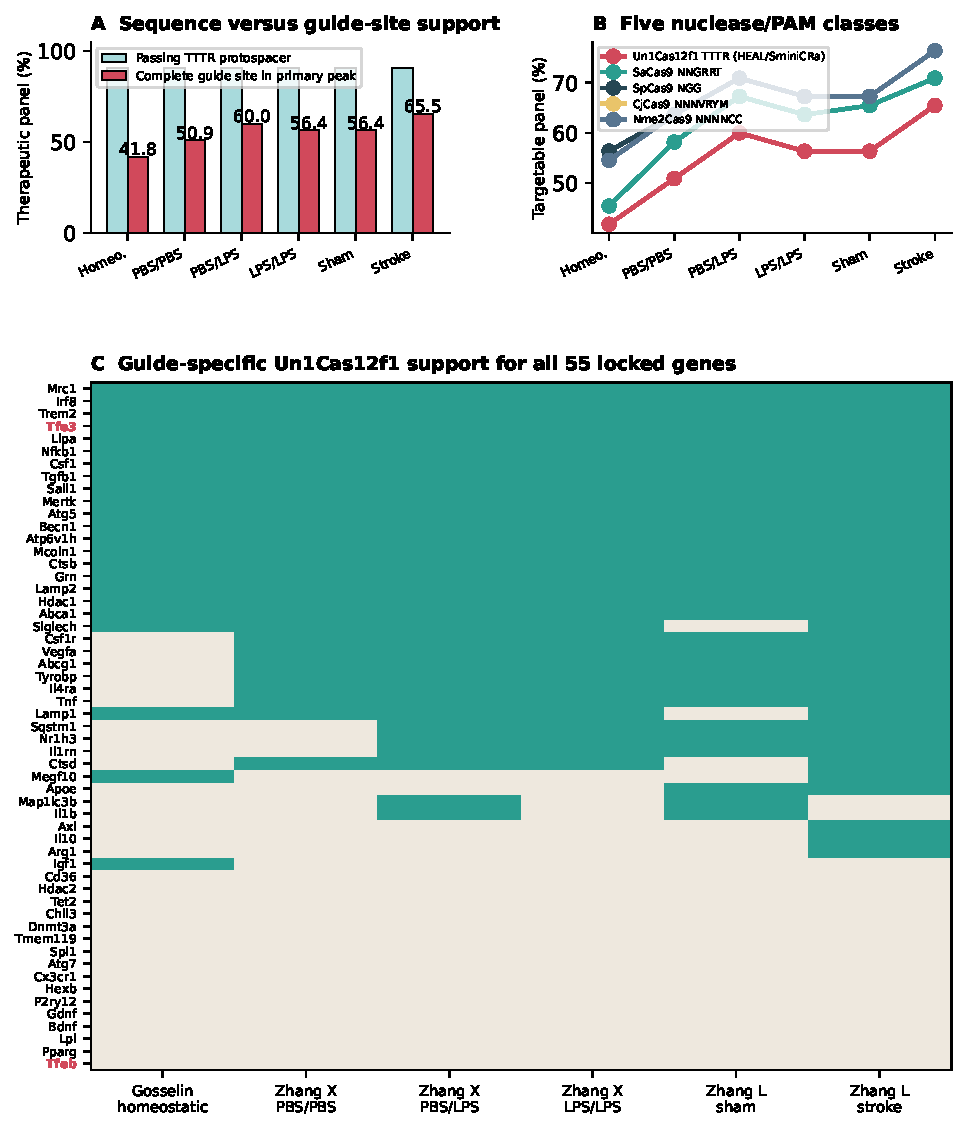
\includegraphics[width=\textwidth]{../figures/output/fig3.pdf}\caption*{Figure 3}\end{figure}
\clearpage
\begin{figure}[p]\centering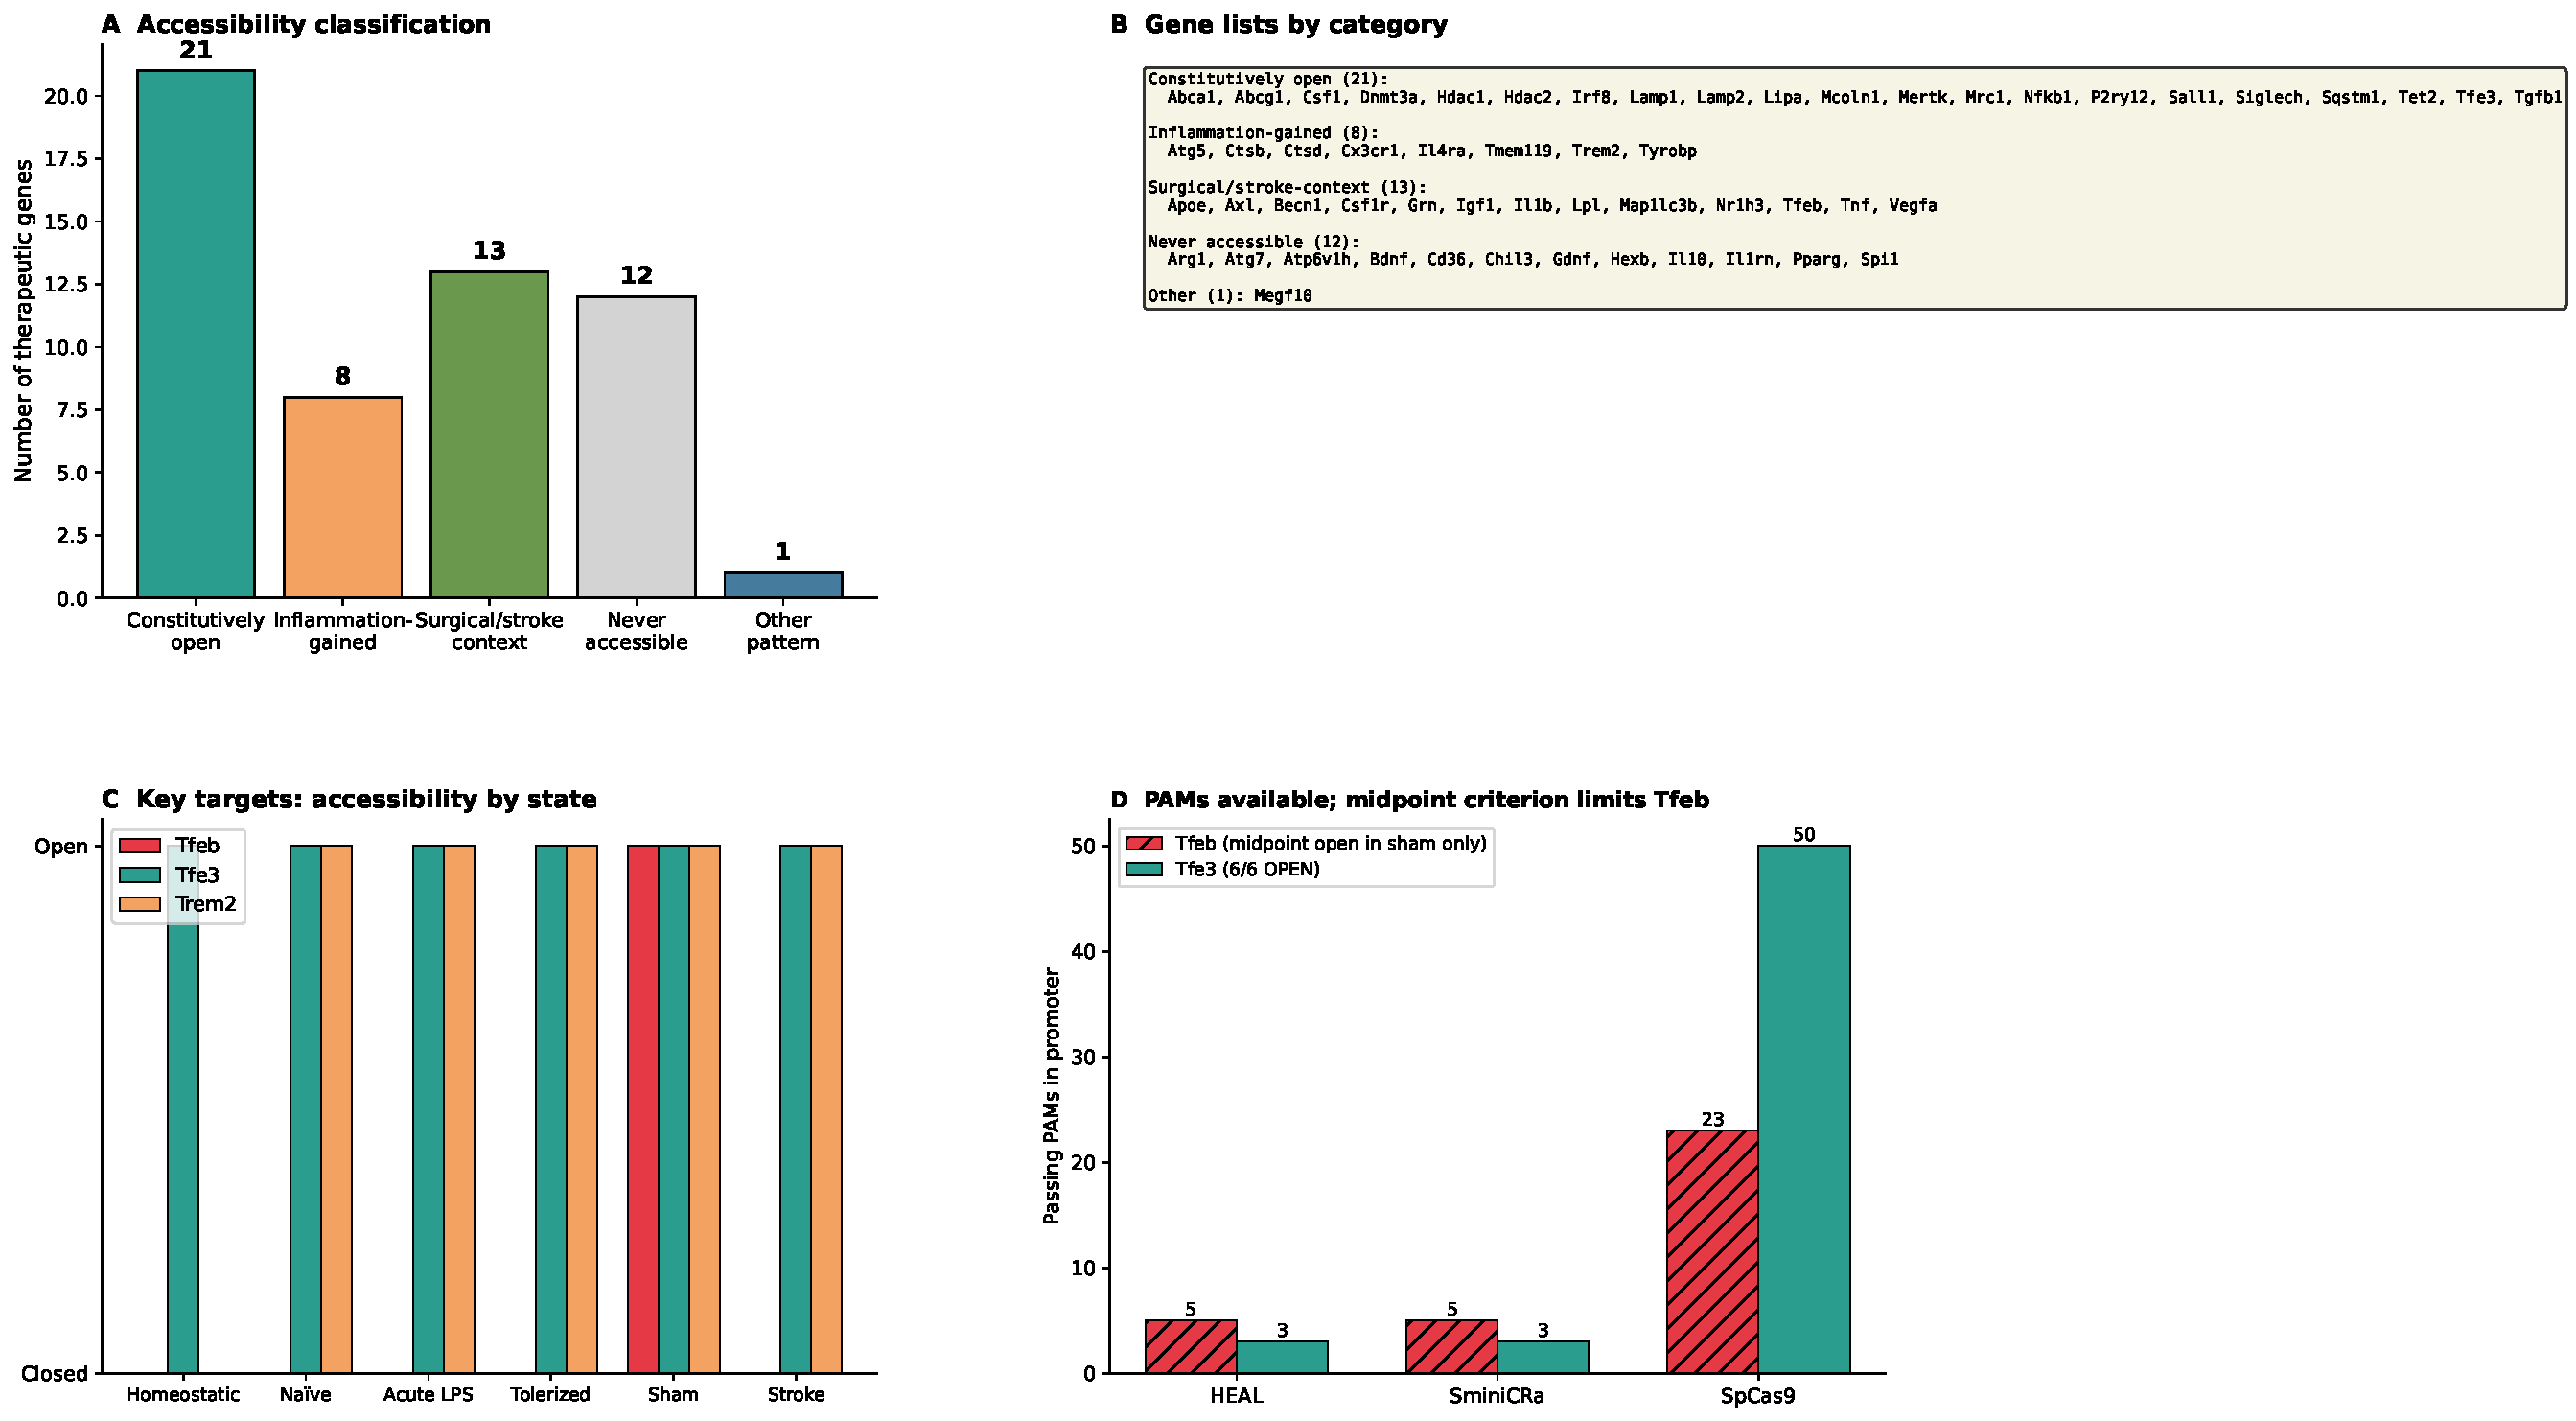
\includegraphics[width=\textwidth]{../figures/output/fig4.pdf}\caption*{Figure 4}\end{figure}
\clearpage
\begin{figure}[p]\centering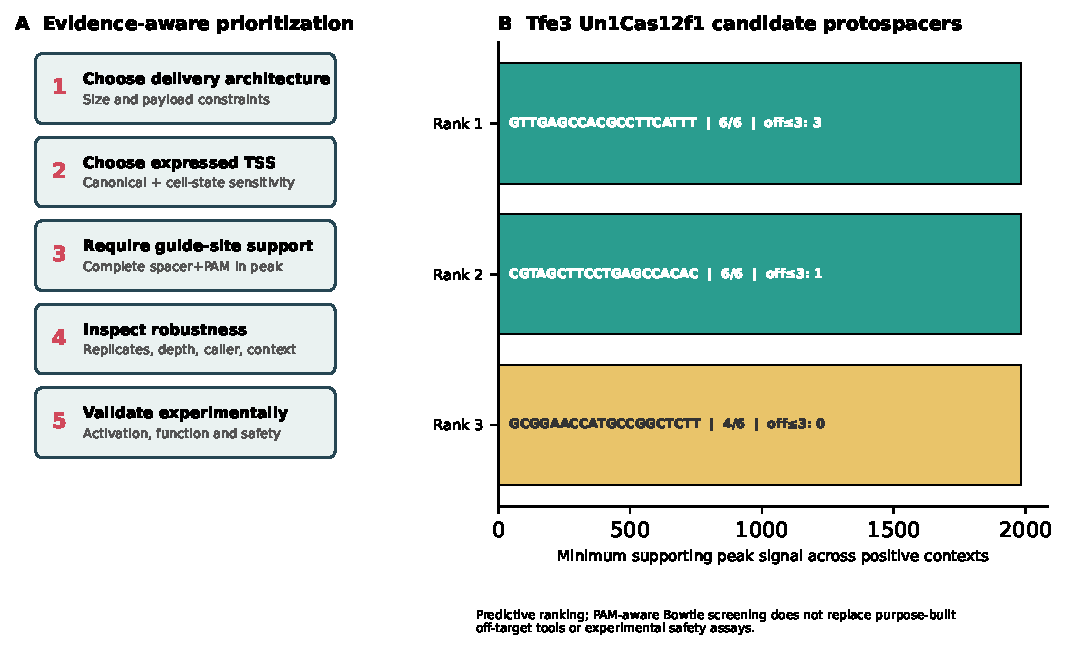
\includegraphics[width=\textwidth]{../figures/output/fig5.pdf}\caption*{Figure 5}\end{figure}
\clearpage
\begin{figure}[p]\centering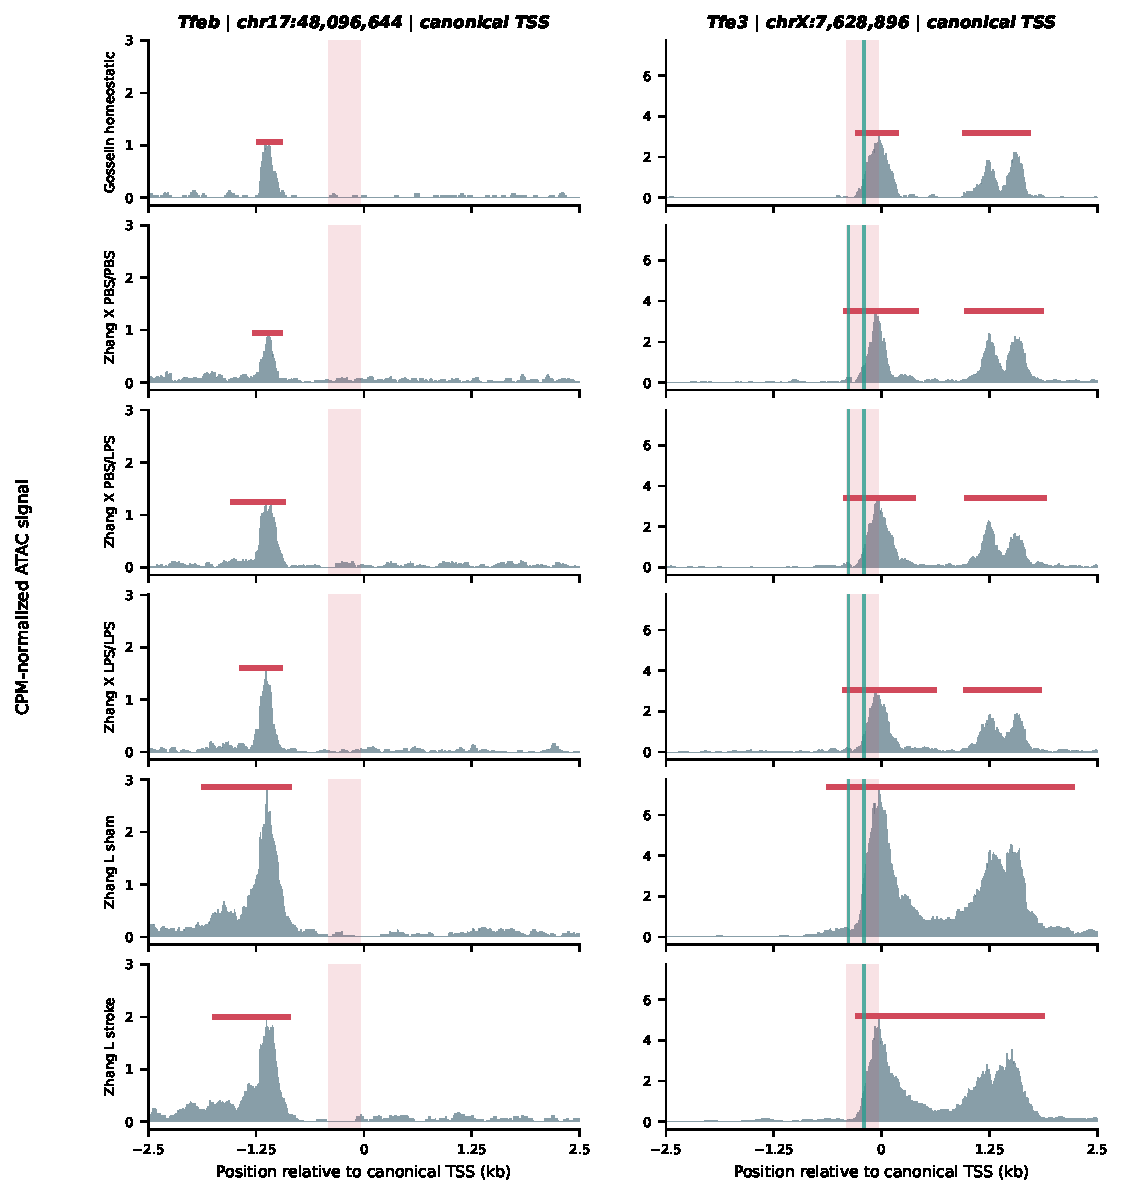
\includegraphics[width=\textwidth]{../figures/output/fig6.pdf}\caption*{Figure 6}\end{figure}

\end{document}
